% !TeX spellcheck = de_DE
\documentclass{uebung_cs}
\usepackage{algo121}
\blattname{Wochenplan: Dijkstras Algorithmus}

%%%%%%%%%%%%%%%%%%%%%%%%%%%%%%%%%%%%%%%%%%%%%%%%%%%%%%%%%%%%%%%%%%%%%%%%%%%%

\begin{document}
\section*{Vorbereitung}
Lies E Kapitel 8 ohne 8.7 (oder CLRS Kapitel 24 ohne 24.1 und 24.4) und schau das Video der Woche.

\section*{Dienstag}
\begin{aufgabe}[Algorithmen und Eigenschaften]\label{tue-first}\mbox{}
	\begin{enumerate}
		\item (\warmup) Gegeben sei der Graph aus Abbildung~\ref{example_graph}.
		Zeige den Baum kürzester Wege für den Graphen (bei Startknoten 0).
		Schreibe die Länge des kürzesten Weges von Knoten 0 zu jedem Knoten.
		\item Gib einen Beispielgraphen an, der negative Kantengewichte aber keine negativen Kreise hat, und der für eine falsche Ausgabe von Dijkstras Algorithmus sorgt.
		\item Gegeben sei nun ein Graph $G$ mit $n$ Knoten und $m$ Kanten, und ein Baum $T$ in $G$, dessen Wurzel Knoten $s$ sei.
		Zeige, wie man in Zeit $\O(n+m)$ feststellt, ob $T$ ein Baum kürzester Wege mit Startknoten $s$ ist.
		\item Sei $T$ ein Baum kürzester Wege von Knoten $s$ in einem Graphen~$G$.
		Ist $T$ immer noch ein Baum kürzester Wege, wenn wir auf alle Kantengewichte eine Konstante $c$ addieren?
	\end{enumerate}
\end{aufgabe}
\begin{figure}[h]
	\begin{center}
		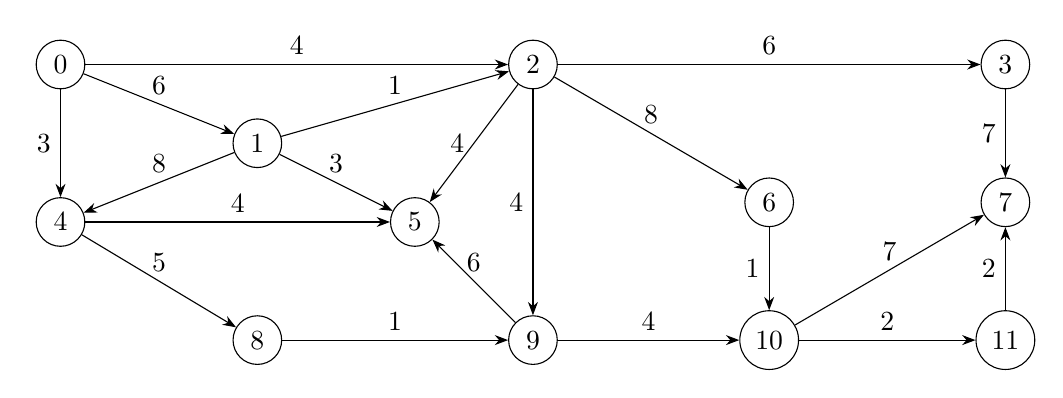
\begin{tikzpicture}
			\usetikzlibrary{arrows.meta}
			\node[draw,circle] (v0)  at (0,  3.5)	{$0$};
			\node[draw,circle] (v1)  at (2.5,2.5)	{$1$};
			\node[draw,circle] (v2)  at (6,  3.5)	{$2$};
			\node[draw,circle] (v3)  at (12, 3.5)	{$3$};
			\node[draw,circle] (v4)  at (0,1.5)	{$4$};
			\node[draw,circle] (v5)  at (4.5,1.5)	{$5$};
			\node[draw,circle] (v6)  at (9,1.75)	{$6$};
			\node[draw,circle] (v7)  at (12,1.75)	{$7$};
			\node[draw,circle] (v8)  at (2.5,0)	{$8$};
			\node[draw,circle] (v9)  at (6,0)	{$9$};
			\node[draw,circle] (v10) at (9,0)	{$10$};
			\node[draw,circle] (v11) at (12,0)	{$11$};
			%
			\def\list {v0/v1/6, v0/v2/4, v1/v2/1, v1/v4/8, v1/v5/3, v2/v3/6, v2/v6/8, v4/v5/4, v4/v8/5, v8/v9/1, v9/v5/6, v9/v10/4, v10/v7/7, v10/v11/2}  % list elements
			\foreach \u\v\weight in \list
			{	\draw[-Stealth] (\u) -- (\v) node [midway, above] {\weight};
			}
			\def\vertical {v0/v4/3, v2/v5/4, v2/v9/4, v3/v7/7, v6/v10/1, v11/v7/2}  % list elements
			\foreach \u\v\weight in \vertical
			{	\draw[-Stealth] (\u) -- (\v) node [midway, left] {\weight};
			}
			%
		\end{tikzpicture}
		\caption{\label{example_graph}Ein gerichteter, gewichteter Beispielgraph.}
	\end{center}
\end{figure}

\begin{aufgabe}[Noch mehr Kabel]
	Die Kabelfernsehen-Firma AlgoMedia überträgt Kabelfernsehen an alle Häuser in Algo-Stadt.
	Sie übermitteln die TV Signale von ihrem Hauptsitz mittels eines Kabelnetzwerks, wobei die Länge jedes Kabels bekannt ist.
	Die Kabel verlaufen zwischen Verteilerkästen:
	Es gibt einen Kasten in jedem Haus, einen Kasten im Hauptsitz der Firma, und sonst keine weiteren Kästen.
	Jeder Kasten ist durch direkte Kabel mit einem oder mehreren anderen Kästen verbunden. Es gibt $X$ Häuser und $K$ Kabel im Netzwerk.

	Löse folgende Aufgaben:
	\begin{enumerate}
		\item AlgoMedia möchte, dass alle Kund:innen das bestmögliche Signal erhalten.
		Die Signalqualität sinkt proportional zur Länge des Kabels.
		Gib einen Algorithmus an, der die Signale so von Kasten zu Kasten leitet, dass die Signalqualität für jeden Empfängerkasten maximiert wird.
		\item Nach genauerer Betrachtung bemerkt AlgoMedia, dass die Qualität eines Signals, wenn es durch einen einzelnen Kasten läuft, genauso sinkt, als hätte es 5 Meter Kabellänge durchlaufen.
		Passe deinen Algorithmus so an, dass er in diesem Szenario die Signale so leitet, dass die Empfangsqualität an jedem Kasten maximiert wird.
		\item Nach Kürzungen von staatlichen Mitteln versucht AlgoMedia, Geld zu sparen und also nur absolut notwendige Kabel zu behalten.
		Aktuell geben sie 42,000 Euro im Jahr für jeden Meter Kabel aus.
		Gib einen Algorithmus an, der die günstigste Möglichkeit berechnet, sodass alle Häuser in Algo-Stadt mit einem Signal versorgt werden können.
	\end{enumerate}
\end{aufgabe}


\begin{aufgabe}[Längster Pfad in gerichteten, kreisfreien Graphen]
	Bestimme einen Algorithmus, um den \emph{längsten} Weg in einem gerichteten, kreisfreien Graphen zu finden.
\end{aufgabe}

\newpage\section*{Donnerstag}
\begin{aufgabe}[Dijkstra und Knotengewichte]
	Sei $G$ ein gerichteter Graph, bei dem alle \emph{Knoten} ein nicht-negatives Gewicht haben.
	Das Gewicht eines Weges in $G$ ist jetzt die Summe der Gewichte der Knoten auf dem Weg.
	Bestimme einen Algorithmus, um den kürzesten Weg zwischen zwei Knoten in $G$ zu bestimmen.
\end{aufgabe}

\begin{aufgabe}[Reiseplanung in Zombiezeiten, \hard]
	Scheinbar hat deine Gruppe es geschafft der brenzligen Zombiesituation des Union-Find Blattes zu entkommen.
	Jetzt müsst ihr den sichersten Weg zwischen zwei Städten finden, um hoffentlich nicht von Zombies gegessen zu werden.
	Der Graph $G$ sei gegeben: Jeder Knoten ist eine Stadt und jede Kante ist eine Straße zwischen zwei Städten. Für jede Kante $e$ gibt es eine Wahrscheinlichkeit $s(e)$ mit $0 \leq s(e) \leq 1$, die angibt, ob man die Benutzung der Straße überlebt.
	Die Wahrscheinlichkeiten für die Kanten sind unabhängig und die Wahrscheinlichkeit, auf einem Pfad $P$ zu überleben, ist das Produkt über die Wahrscheinlichkeiten der einzelnen Kanten.
	\begin{center}
	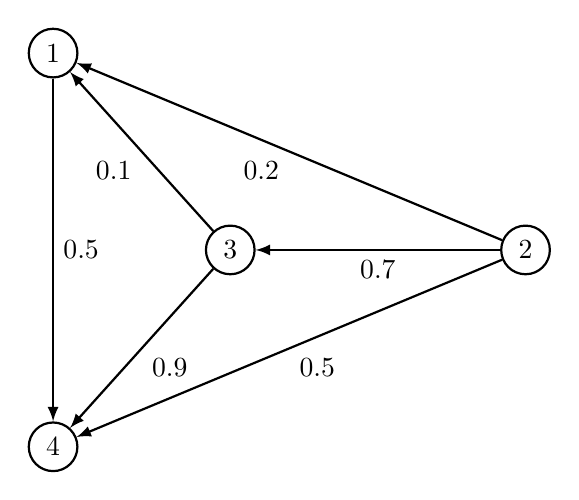
\begin{tikzpicture}[-latex, thick, auto]
		\tikzstyle{vertex} = [circle, draw]
		\node[vertex](A) at (0,5) {1};
		\node[vertex](B) at (2.25,2.5) {3};
		\node[vertex](C) at (6,2.5) {2};
		\node[vertex](D) at (0,0) {4};
		\path  (B) edge node {0.1} (A);
		\path  (B) edge node {0.9} (D);
		\path  (C) edge node {0.7} (B);
		\path  (C) edge node {0.5} (D);
		\path  (C) edge node {0.2} (A);
		\path  (A) edge node {0.5} (D);
	\end{tikzpicture}
	\end{center}
	Wenn man in diesem Beispiel direkt von Knoten 2 zu Knoten 4 geht, hat man eine Wahrscheinlichkeit von 50\%, zu überleben.
	Wenn man aber den Pfad $2\rightarrow 3 \rightarrow 4$ nimmt, hat man eine Wahrscheinlichkeit von $0.7\cdot 0.9 = 0.63 = 63\%$, zu überleben.
	Entwirf einen Algorithmus, der für einen beliebigen, gegebenen Eingabegraphen den sichersten Weg zwischen zwei Knoten $s$ und $t$ bestimmt.
\end{aufgabe}

\begin{aufgabe}[Tiefhängende Äste]
	Eine \emph{Weide} ist ein gewichteter, gerichteter Graph, den man aus einem Binärbaum erhält, indem man für jedes Blatt jeweils eine zur Wurzel gerichtete Kante einfügt.
	Alle Kanten haben nicht-negative Gewichte.
	% Hier tikz Zaubereien
	\begin{center}
		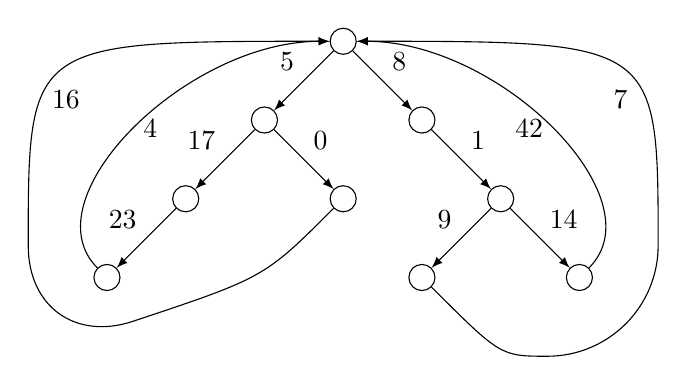
\begin{tikzpicture}
			\usetikzlibrary{arrows.meta}
			%
			\def\nodes {root/0/3, l/-1/2, ll/-2/1, lr/0/1, lll/-3/0, r/1/2, rr/2/1, rrl/1/0, rrr/3/0};
			% leaves: lll, lr, rrl, rrr
			% draw nodes of the weide
			\foreach \label\x\y in \nodes{
				\node[draw,circle] (\label) at (\x,\y) {};
			}
			% draw ``inner'' edges of the weide
			\def\edges {root/l/left/5, l/ll/left/17, l/lr/right/0, ll/lll/left/23, root/r/right/8, r/rr/right/1, rr/rrl/left/9, rr/rrr/right/14};
			\foreach \s\t\labelside\weight in \edges{
				\draw[-latex] (\s) -- (\t) node[midway, above \labelside] {$\weight$};
			}
			% draw bendy bendy edges from leaves to wurzel of the weide
			\draw[-latex] 
				(lll) 
				.. controls (-4,1) and (-2,3) 
				.. (root)
			node [midway, right] {$4$};
			\draw[-latex, rounded corners=40] 
				(lr)
				.. controls (-1,0) 
				.. (-4,-1)
				.. controls (-4,3)
				.. (root)
			node [midway, below] {$16$};
			\draw[-latex] 
				(rrr) 
				.. controls (4,1) and (2,3) 
				.. (root)
			node [midway, left] {$42$};
			\draw[-latex, rounded corners=40] 
				(rrl)
				.. controls (2,-1) 
				.. (4,-1)
				.. controls (4,3)
				.. (root)
			node [midway, below] {$7$};
		\end{tikzpicture}
	\end{center}
	Betrachte eine Weide mit $n$ Knoten.
	Wir wollen für einen gegebenen Knoten $s$ die kürzesten Wege zu allen anderen Knoten ermitteln.
	\begin{enumerate}
		\item Wie lange braucht Dijkstras Algorithmus, um dieses Problem zu lösen?
		Gib die Laufzeit als Funktion von $n$ an.
		\item (\hard) Entwirf einen schnelleren Algorithmus. 
	\end{enumerate} 
\end{aufgabe}

\end{document}
